\chapter{Experimental Evaluation}

In this chapter, we assess the potential benefit of using SecureWilly in docker projects. Through a variety of experiments, we display the results of SecureWilly's execution, we examine the profiles produced and we evaluate the performance, the functionality and the scalability of our software.

\section{Experimental setup}\label{expset}
\subsection{Benchmarks}
SecureWilly has been tested on creating AppArmor profiles for a set of multi-service projects provided by CloudSuite, a benchmark suite for cloud services. \cite{cloudsuite} The benchmarks are based on real-world software stacks and represent real-world setups. 

\begin{description}[style=nextline]
\item[Media Streaming]
One of the benchmarks of Cloudsuite that was used in the experimental evaluation was media-streaming. This benchmark uses the Nginx web server as a streaming server for hosted videos of various lengths and qualities. The client, based on httperf's wsesslog session generator, generates a request mix for different videos, to stress the server. \cite{mediastr}

The benchmark has two tiers: the server and the clients. The server runs Nginx, and the clients send requests to stream videos from the server. Each tier has its own image which is identified by its tag.

The streaming server requires a video dataset to serve and a synthetic dataset is generated, comprising several videos of different lengths and qualities. A separate docker image that handles the dataset generation is provided, which is then used to launch a dataset container that exposes a volume containing the video dataset.

To facilitate the communication between the client(s) and the server, a docker network is built, and the launched containers were attached to it.

\item[Data-Caching]
Another benchmark of CloudSuite that was used in our experimental evaluation was data-caching. This benchmark uses the Memcached data caching server, simulating the behavior of a Twitter caching server using a twitter dataset. The metric of interest is throughput expressed as the number of requests served per second. The workload assumes strict quality of service guarantees. \cite{datacaching}

This benchmark features two tiers: the server(s), running Memcached, and the client(s), which request data cached on the Memcached servers. Each tier has its own image which is identified by its tag.

To facilitate the communication between the client(s) and the server, a docker network is built, and the launched containers were attached to it.
\end{description}

In the following instances, the benchmarks were executed, having one client and one server. SecureWilly produced one profile for each of the services of every benchmark.

\subsection{Nextcloud}

Despite the fact that CloudSuite's benchmarks are based on real-world software, we considered testing a real program, which is widely used and a lot of users rely on docker images in order to run it, and exercise it first-hand. Our choice was Nextcloud.

\begin{figure}[h!]
  \centering
   
\includegraphics[width=0.3\linewidth]{../figures/Nextcloud.png}
   \caption{Nextcloud's trademark}
\end{figure}

Nextcloud is a suite of client-server software for creating and using file hosting services. It is free and open-source, which means that anyone is allowed to install and operate it on their own private server devices. \cite{wikinext}

Although it is true that Nextcloud offers a variety of operations (file sharing, communication etc), we will be using it in its simplest form, where Nextcloud is used to run a personal cloud storage service, making files accessible via the internet and sharing them with other users.

The services of Nextcloud's project in the particular example are two:
\begin{enumerate}
\item \textbf{db}, which is actually the database used for data storage - in our case, we chose a MySQL/MariaDB database
\item \textbf{nextcloud}, which is the server of this docker project
\end{enumerate}

The docker-compose file which was used as input to SecureWilly's UI is the following (options security\_opt and container name were added by SecureWilly):

\begin{lstlisting}[style=Dockerfile, caption={Nextcloud's docker-compose.yml}]
version: '3'

volumes:
     nextcloud_:
     db_:

services:
     db:
        container_name: db
        security_opt:
          - "apparmor:db_profile"
        image: mariadb:10
        command: --transaction-isolation=READ-COMMITTED --binlog-format=ROW
        restart: always
        volumes:
                - db_:/var/lib/mysql
        environment:
                - MYSQL_ROOT_PASSWORD=secret
                - MYSQL_PASSWORD=secret
                - MYSQL_DATABASE=nextcloud_
                - MYSQL_USER=willy
     nextcloud:
        container_name: nextcloud
        security_opt:
          - "apparmor:nextcloud_profile"
        image: nextcloud
        ports:
                - 8080:80
        links:
                - db
        volumes:
                - nextcloud_:/var/www/html
                - /home/ubuntu/SecureWilly/Nextcloud/data:
					/var/www/html/data
        environment:
                - NEXTCLOUD_ADMIN_USER=willy
                - NEXTCLOUD_ADMIN_PASSWORD=secret
                - NEXTCLOUD_TABLE_PREFIX=nc_
                - NEXTCLOUD_DATA_DIR=/var/www/html/data
        restart: always
\end{lstlisting}

The Nextcloud installation and all data beyond what lives in the database (file uploads, etc) is stored in the docker volume /var/www/html. The docker daemon will store that data within the docker directory /var/lib/docker/volumes/. This keeps data persistent, meaning it is saved even if the container crashes, is stopped or deleted.

The volumes used in the yml file are the following:
\begin{itemize}
\item /var/www/html: Main folder, needed for updating
\item /var/www/html/data: The actual data of your Nextcloud
\item /var/lib/mysql: Database's volume
\end{itemize}

The test plan, which we provided as input, was minimal as it included some configuration commands for nextcloud's server and uploading a file to the cloud storage:

\begin{lstlisting}[style=bashscript, caption={Test plan used in Nextcloud's project}]
#Clear data directory if it exists and chown it to www-data, as configured in Nextcloud
sudo rm -r /home/ubuntu/SecureWilly/Nextcloud/data
mkdir /home/ubuntu/SecureWilly/Nextcloud/data
sudo chown www-data:www-data /home/ubuntu/SecureWilly/Nextcloud/data

#Start the containers
docker-compose up -d

#Wait some time for the database to be configured
sleep 60

#Check server's status
docker exec -u www-data nextcloud php occ status > answer
answer=$(cat answer | grep 'Nextcloud is not installed')
while [ -z "$answer" ] && [ ! -z "$error_exec" ]
do
        rm answer
        docker exec -u www-data nextcloud php occ status > answer 2> error_exec
        answer=$(cat answer | grep 'Nextcloud is not installed')
		  error_exec=$(cat answer | grep 'is not running')
done
rm answer

#Configure nextcloud, when the server is up
docker exec -u www-data nextcloud php occ maintenance:install --database "mysql" --database-name "nextcloud_" --database-host "db" --database-user "willy" --database-pass "secret" --admin-user "willy" --admin-pass "secret"

#Create a file in local data directory
sudo touch /home/ubuntu/SecureWilly/Nextcloud/data/willy/files/HelloFromTheOtherSide

#Use occ files:scan to make it visible to the web interface
docker exec -u www-data nextcloud php occ files:scan --all

#Stop the containers when you're finished
docker kill nextcloud
docker kill db
\end{lstlisting}

\section{Profiles}
\subsection{SecureWilly's profiles}
After SecureWilly's execution, the final AppArmor profiles are produced and are already loaded in kernel. The final profiles are under \textit{parser\_output} directory.

Nextcloud's services profiles are presented below as an example. The following profiles were created by SecureWilly on a VM launched in OpenStack using an image of Ubuntu 16.04 and also tested on Arch Linux.

\begin{lstlisting}[style=Dockerfile, caption={AppArmor profile for db service: db\_profile}]
#include <tunables/global>

profile db_profile flags=(attach_disconnected,mediate_deleted) {
        capability setgid,
        capability dac_override,
        network inet dgram,
        /var/lib/mysql/* rw,
        signal (receive) set=(term) peer=db_profile,
        mount /var/lib/docker/volumes/nextcloud_db_/_data -> /var/lib/mysql, #Bind host to docker volume
        signal (send) set=(usr1) peer=db_profile,
        file,  #Allows access to containers filesystem
        /var/lib/docker/* r, #Access to layers of filesystem
        network inet6 stream,
        signal (receive) set=(kill) peer=unconfined,
        deny remount /var/lib/mysql, #Disallow remounting this mountpoint
        network inet6 dgram,
        signal (receive) set=(usr1) peer=db_profile,
        deny umount /var/lib/mysql, #Disallow breaking this mountpoint
        capability setuid,
        signal (send) set=(term) peer=db_profile,
        deny ptrace (readby, tracedby), #Confront container breakout attacks
}
\end{lstlisting}

\begin{lstlisting}[style=Dockerfile, caption={AppArmor profile for nextcloud service: nextcloud\_profile}]
#include <tunables/global>

profile nextcloud_profile flags=(attach_disconnected,mediate_deleted) {
        /var/www/html/data/* rw,
        capability fsetid,
        capability chown,
        file,  #Allows access to containers filesystem
        mount /var/lib/docker/volumes/nextcloud_nextcloud_/_data -> /var/www/html, #Bind host docker volume
        network inet6 dgram,
        signal (receive) set=(exists) peer=unconfined,
        mount /home/ubuntu/SecureWilly/Nextcloud/data -> /var/www/html/data, #Bind host to docker volume
        network inet stream,
        /var/www/html/* rw,
        /var/lib/docker/* r, #Access to layers of filesystem
        network inet6 stream,
        capability fowner,
        capability setgid,
        signal (receive) set=(usr2) peer=nextcloud_profile,
        capability dac_override,
        deny umount /var/www/html, #Disallow breaking mntpnt
        signal (send) set=(usr2) peer=nextcloud_profile,
        deny remount /var/www/html/data, #Disallow remounting this mountpoint
        network inet dgram,
        capability setuid,
        deny remount /var/www/html, #Disallow remounting this mountpoint
        deny ptrace (readby, tracedby), #Confront container breakout attacks
        capability net_bind_service,  #This capability is needed to bind a socket to well-known ports
        signal (receive) set=(kill) peer=unconfined,
        deny umount /var/www/html/data, #Disallow breaking mntpnt
}
\end{lstlisting}

Although the profiles produced are mainly service-oriented there are still some rules that depend on host's paths and configuration.

One of them is a mount rule, where the host path is needed in order to have a strict rule indicating the mount of a particular volume.

Except for the mount rules, through testing we came to the conclusion that host's system can also affect the AppArmor profile of a service. For example, the way a host treats the networking of containers may differ from one machine to another and therefore, new network rules may be required.

The same Nextcloud instance was tested again on another host, using an image of Ubuntu 18.10 and the following profiles were created by SecureWilly. The following profiles defer from the previous one on network rules, as they needed some extra networking using unix stream and netlink raw.

\begin{lstlisting}[style=Dockerfile, caption={New AppArmor profile for db service: db\_profile}]
#include <tunables/global>

profile db_profile flags=(attach_disconnected,mediate_deleted) {
	capability dac_override,
	network inet dgram,
	/var/lib/mysql/* rw,
	network unix stream,
	signal (receive) set=(term) peer=db_profile,
	signal (receive) set=(usr1) peer=db_profile,
	signal (send) set=(term) peer=db_profile,
	signal (send) set=(usr1) peer=db_profile,
	file,  #Allows access to containers filesystem
	/var/lib/docker/* r, #Access to layers of filesystem
	network inet6 stream,
	signal (receive) set=(kill) peer=unconfined,
	deny remount /var/lib/mysql, #Disallow remounting this mountpoint
	network inet6 dgram,
	mount /var/lib/docker/volumes/nextcloud_db_/_data -> /var/lib/mysql, #Bind host to docker volume
	capability setgid,
	deny umount /var/lib/mysql, #Disallow breaking this mountpoint
	capability setuid,
	network netlink raw,
	deny ptrace (readby, tracedby), #Confront container breakout attacks
}
\end{lstlisting}
\clearpage
\begin{lstlisting}[style=Dockerfile, caption={New AppArmor profile for nextcloud service: nextcloud\_profile}]
#include <tunables/global>

profile nextcloud_profile flags=(attach_disconnected,mediate_deleted) {
	/var/www/html/data/* rw,
	network unix stream,
	capability chown,
	file,  #Allows access to containers filesystem
	network inet6 dgram,
	signal (receive) set=(exists) peer=unconfined,
	network netlink raw,
	mount /home/fani/SecureWilly/Nextcloud/data -> /var/www/html/data, #Bind host to docker volume
	mount /var/lib/docker/volumes/
		nextcloud_nextcloud_/_data -> /var/www/html, #Bind host to docker volume
	network inet stream,
	/var/www/html/* rw,
	/var/lib/docker/* r, #Access to layers of filesystem
	network inet6 stream,
	capability fowner,
	capability setgid,
	signal (receive) set=(usr2) peer=nextcloud_profile,
	capability dac_override,
	deny umount /var/www/html, #Disallow breaking this mountpoint
	signal (send) set=(usr2) peer=nextcloud_profile,
	deny remount /var/www/html/data, #Disallow remounting this mountpoint
	network inet dgram,
	capability setuid,
	deny remount /var/www/html, #Disallow remounting this mountpoint
	deny ptrace (readby, tracedby), #Confront container breakout attacks
	capability net_bind_service,  #This capability is needed to bind a socket to well-known ports
	signal (receive) set=(kill) peer=unconfined,
	deny umount /var/www/html/data, #Disallow breaking this mountpoint
}
\end{lstlisting}
\begin{mdframed}[backgroundcolor=navajowhite]
To sum up, SecureWilly's profiles are service-oriented but they still have some dependencies from the host machine, like mount rules and host's configuration on containers. Therefore, it is not recommended to use a profile coming from another system, but run SecureWilly to create a profile adjusted to your system.
\end{mdframed}

\subsection{Genprof profile comparison}\label{genprofcompare}
Although SecureWilly's profiles have some dependencies from the host, they are not host-oriented in the way a profile created by genprof tool is. Below, we created a profile via genprof for the same Nextcloud instance in order to spot the differences.

The profile was created using the following command:

\begin{lstlisting}[style=dockercommands]
$ sudo aa-genprof ./genprof_run.sh
\end{lstlisting}

The \textit{genprof\_run.sh} is the same test plan of Nextcloud we mentioned in section \textit{Experimental setup \ref{expset}}.

\begin{lstlisting}[style=Dockerfile, caption={New AppArmor profile for nextcloud service: nextcloud\_profile}]
#include <tunables/global>

/home/fani/SecureWilly/Nextcloud/Genprof_testing/genprof_run.sh {
  #include <abstractions/authentication>
  #include <abstractions/base>
  #include <abstractions/bash>
  #include <abstractions/consoles>
  #include <abstractions/nameservice>
  #include <abstractions/postfix-common>
  #include <abstractions/ubuntu-browsers.d/plugins-common>
  #include <abstractions/user-tmp>
  #include <abstractions/wutmp>

  capability audit_write,
  capability net_admin,
  capability sys_resource,

  /bin/cat mrix,
  /bin/grep mrix,
  /bin/rm mrix,
  /bin/sleep mrix,
  /etc/sudoers r,
  /etc/sudoers.d/README r,
  /home/fani/SecureWilly/Nextcloud/Genprof_testing/genprof_run.sh r,
  /lib/x86_64-linux-gnu/ld-*.so mr,
  /proc/stat r,
  /proc/sys/kernel/cap_last_cap r,
  /proc/sys/kernel/hostname r,
  /proc/sys/net/core/somaxconn r,
  /usr/bin/docker mrix,
  /usr/bin/sudo mrix,
  /usr/local/bin/docker-compose mrix,
  owner /etc/default/locale r,
  owner /etc/environment r,
  owner /etc/sudoers.d/ r,
  owner /home/*/SecureWilly/Nextcloud/Genprof_testing/answer rw,
  owner /proc/*/stat r,
  owner /proc/filesystems r,
  owner /proc/sys/kernel/ngroups_max r,
  owner /{usr/,}lib{,32,64}/** mr,
}
\end{lstlisting}
\hfill\break

\textbf{\underline{Comparison}}
\hfill\break

It is evident that there are a lot of different rules between the profile created by genprof and the ones created by SecureWilly.

First of all, let it be clear that this profile is not going to work as security-opt option in Docker compose or runtime flag on a container. It will not let the container start at all, simply because the \say{file} rule is missing.

Moreover, the host oriented behaviour is evident in genprof's profile, since there is an amount of file rules concerning files and paths on host's machine, even about the docker engine and docker compose itself, which run on the host. All of the rules in genprof's profile refer to the procedure - access and permissions - of running the script which includes the commands of the test plan.

On the other hand, SecureWilly's profiles refer exclusively to the operations inside the container and divide accesses and capabilities to services, depending on the task of each service, so that not all services are allowed to act in the same way. This is of utmost importance, because we have full control of the docker services and no concerns about the rules needed for host in order to setup the services. Each service has a more clear view on what it is allowed to do and each one is restricted at a different rate.

Furthemore, genprof's profile includes several other profiles, due to similar behaviour detected in dynamic analysis. This constitutes the profile generic and not adjusted to the specific project like SecureWilly's profiles are and it definitely is contrary to the Principle of Least Privilege, that we intend to follow, as the included profiles may consist of redundant rules that are not actually needed in our project.

All in all, in the light of the above it is clear that SecureWilly's profiles are more specific, more strict and focused on the task of each service and therefore, they provide full control over a docker project in a more efficient and user friendly way.

\section{AppArmor Overhead}

The benefits deriving from enforcing AppArmor profiles have been explained thoroughly up to this point. The question that reasonably arises after this, is whether the usage of an AppArmor profile will delay our services and decrease the whole project's performance. 

The answer to this question is yes, it does slow down the project. However, the extent to which it does, depends on what the services to profile do. For example, file system accesses are slower than other operations, because they have to be checked. Though, if a process does not open files or sockets, then it should not be affected at all (after initialization). But even file system accesses have such a slight delay on the services, that it is not even noticeable.

The AppArmor was created on top of the idea that users should not notice AppArmor at all and thus, the performance is not affected noticeably by AppArmor.

Using Nextcloud's instance as an example, we compared the time needed to run the test plan when the containers were running unconfined and when the profiles produced by SecureWilly were enforced. The results are diplayed in the figure below.

\begin{figure}[h!]
  \centering
   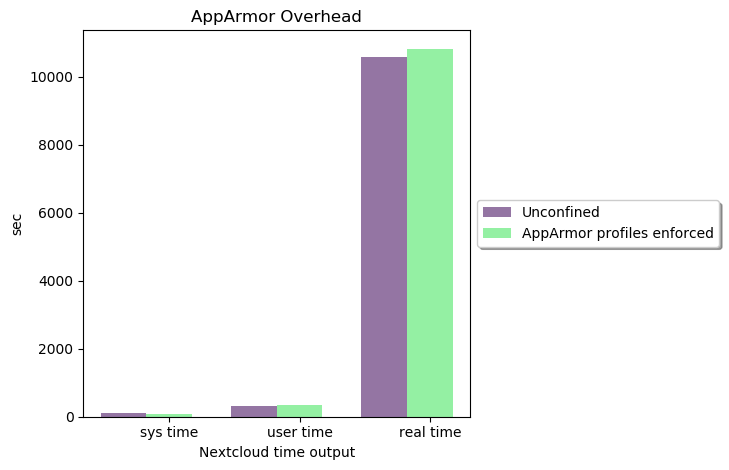
\includegraphics[width=1\linewidth]{../figures/overhead.png}
   \caption{AppArmor overhead}
\end{figure}

It is clear that the overhead of AppArmor is so small that the performance is not affected. Therefore, it is recommended to use AppArmor to harden the security, even if the performance is critical for your project.

\clearpage
\section{Performance}

\underline{Computational complexity}
\hfill\break

In order to evaluate the performance of SecureWilly, we will first find out its computational complexity.

\begin{itemize}
\item First, it is clear that the computational complexity of static analysis is $\mathcal{O}(1)$, because all the operations are about text editing on the input files.
\item Dynamic analysis depends on the computational complexity of the given test plan, which will be repeated $m$ times.

\item Suppose that the computational complexity of the test plan is $f(n)$.

\item As for the computational complexity of the process to set the AppArmor profile in complain or enforce mode, it is represented by a constant $c$, as it takes standard time.

\item Thus, the computational complexity of dynamic analysis is $m*f(n) + c$.

\item The computational complexity of SecureWilly on the whole is

$T(n) = \mathcal{O}(1) + m*f(n) + c \Rightarrow T(n) = m*f(n) + d \Rightarrow T(n) = m*f(n) \Rightarrow T(n) = f(n)$

\end{itemize}

It becomes evident, that the performance of SecureWilly over each benchmark cannot be evaluated using the execution time of SecureWilly, as every test plan has different computational complexity.

Therefore, we approached the performance evaluation by monitoring the amount of runs of each test plan, not by the whole time it took SecureWilly to produce the profiles.

\hfill\break
\underline{Rules per run}
\hfill\break

In Figure 5.3, a line graph illustrates the amount of rules of each service's profile over the test plan runs, referring to media streaming benchmark.

\begin{figure}[h!]
  \centering
   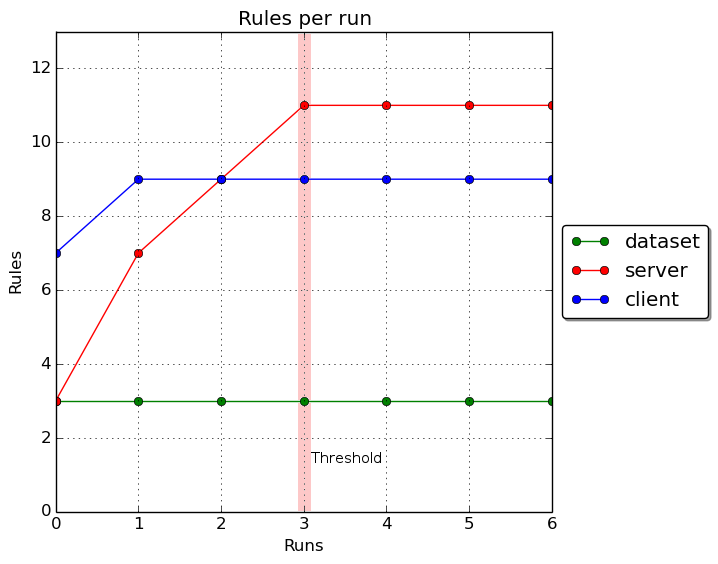
\includegraphics[width=0.70\linewidth]{../figures/mediastreaming/rulesthreshold.png}
   \caption{Media Streaming: Rules per run for each service}
\end{figure}

All of the services start with non-zero amount of rules, which derives from static analysis's preliminary profiles.

We observe that most of the services had a gradual increase in their AppArmor profiles' rules, except for dataset, which starts with a preliminary profile of three rules and remains stable for the rest of the runs. This behaviour of dataset's profile is expected as the corresponding container does not execute any operations, but it only exists in order to expose a volume.

Server's and client's profiles follow a similar escalation, as they both rise to a point and then stabilize over the last runs. The rising derives from the first complain runs, in which rules are extracted gradually, as the addition of some rules leads to new system logs. While the first runs are crucial, as the most part of the rules are extracted over the first runs, the logs become gradually fewer over the last runs until all actions are allowed, and this explains the final stability of the profiles after some runs, as shown in the graph.

Server's shoot up is more enduring and considerable than the client's. This is reasonable, since a server is expected to be responsible for more operations than a client.  

It appears that there is a threshold in runs, which represents the minimum number of runs which have to be executed, until all of the project's profiles stabilize over runs. The threshold for media streaming, as shown in the graph, is at run three. After the threshold, it takes three runs for SecureWilly to finish its execution.

\begin{figure}[h!]
  \centering
   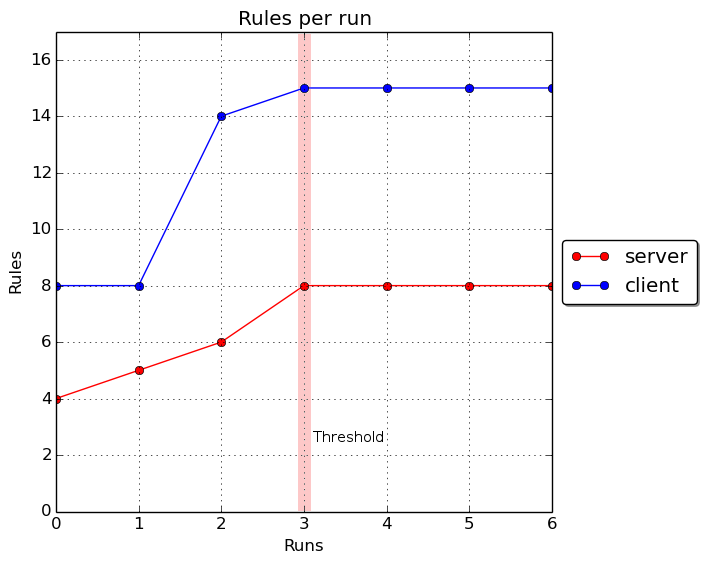
\includegraphics[width=0.70\linewidth]{../figures/datacaching/rulesthreshold.png}
   \caption{Data Caching: Rules per run for each service}
\end{figure}

Figure 5.4 shows the corresponding line graph of data caching benchmark.

Similar to media streaming, both server and client lift to a point and afterwards they remain stable. The threshold we observed before, is at the third run again. Moreover, in this benchmark, server and client traverse the threshold exactly at the same runs.

On the contrary, data caching seems to have more active clients, as client's profile has more rules.

In Figure 5.5, the graph outlines the behaviour of nextcloud's profiles over runs. The threshold in nextcloud's execution is at run four. This slight difference with CloudSuite's benchmarks is reasonable, as nextcloud's server appears to need more rules in its profile, in order to complete its operations. Thus, SecureWilly needs to execute more runs of the test plan in order to extract all the rules necessary.

Nextcloud's server and database service traverse the threshold almost at the same run, and their escalation is quite similar. Server's service though requires more rules in its profile, as it commits more actions, comparing to the database.

\begin{figure}[h!]
  \centering
   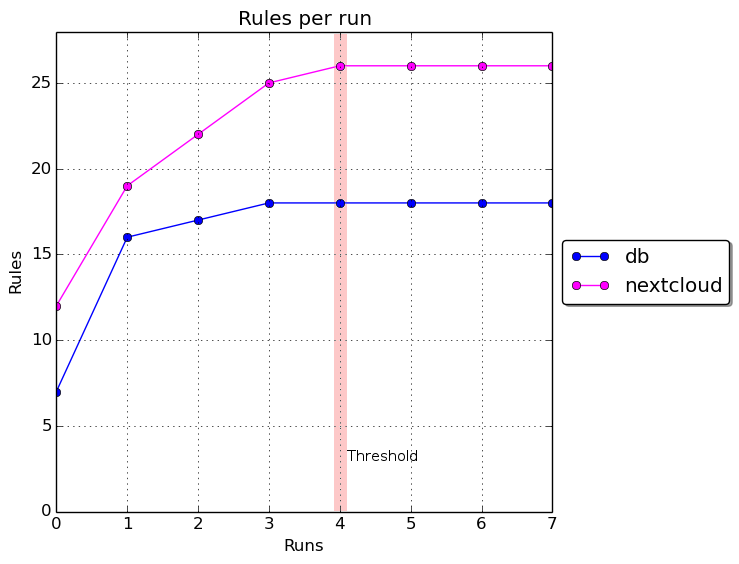
\includegraphics[width=0.75\linewidth]{../figures/nextcloud/rulesthreshold.png}
   \caption{Nextcloud: Rules per run for each service}
\end{figure}
\hfill\break

The bar chart, in figure 5.6, depicts the performance of SecureWilly on every project, by diplaying the amount of runs of the test plan and the run that consistutes the last augmentation in services' profiles, given by the value of threshold.

\begin{figure}[h!]
  \centering
   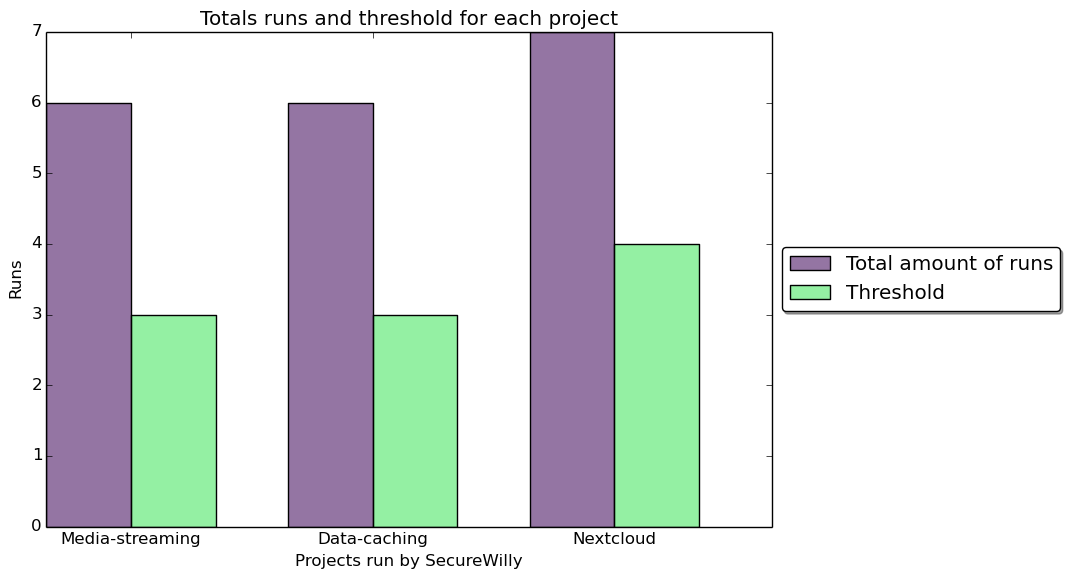
\includegraphics[width=1\linewidth]{../figures/compare.png}
   \caption{Comparing total runs and threshold between projects run by SecureWilly}
\end{figure}

It becomes evident, that the performance of SecureWilly on each project depends on the complexity of the project and the amount of operations that the test plan executes, which will lead to the amount of runs it needs, until it reaches its threshold. The threshold is set also based on the complexity of the project.

\hfill\break
\underline{Time of test plan per run}
\hfill\break

As described above, comparing the execution time between different projects run by SecureWilly is meaningless. The only essential way to observe time would be monitoring the time execution of test plan over runs.

Figures 5.7, 5.8 and 5.9 represent the line graphs of each project, which illustrate the execution time of the test plan over runs executed by SecureWilly.

The execution time was captured by executing the time command on the run script of dynamic parser. To calculate the execution time, we used the sum of sys and usr time, which shows the actual CPU time that docker containers' processes used.

\begin{figure}[h!]
  \centering
   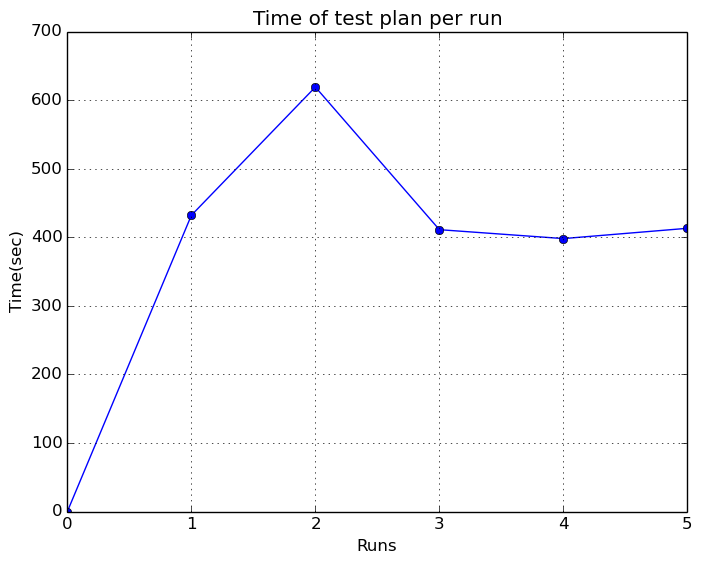
\includegraphics[width=0.70\linewidth]{../figures/mediastreaming/time.png}
   \caption{Media Streaming: Time of test plan per run}
\end{figure}

\begin{figure}[h!]
  \centering
   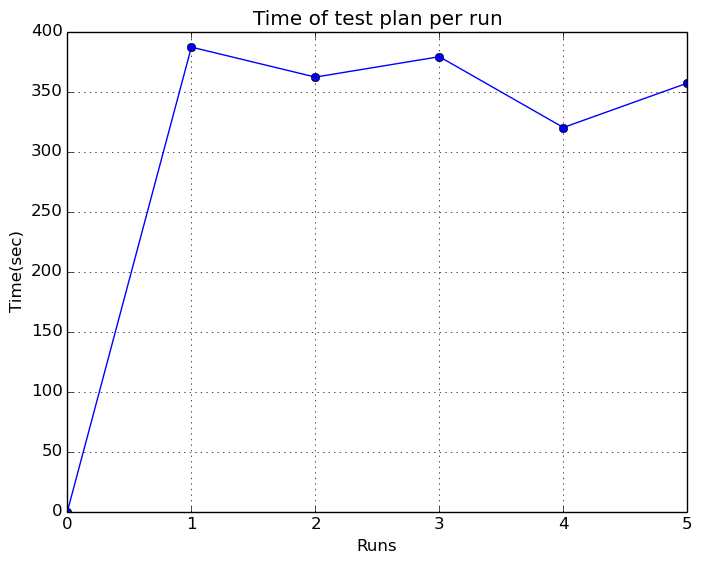
\includegraphics[width=0.70\linewidth]{../figures/datacaching/time.png}
   \caption{Data Caching: Time of test plan per run}
\end{figure}

\begin{figure}[h!]
  \centering
   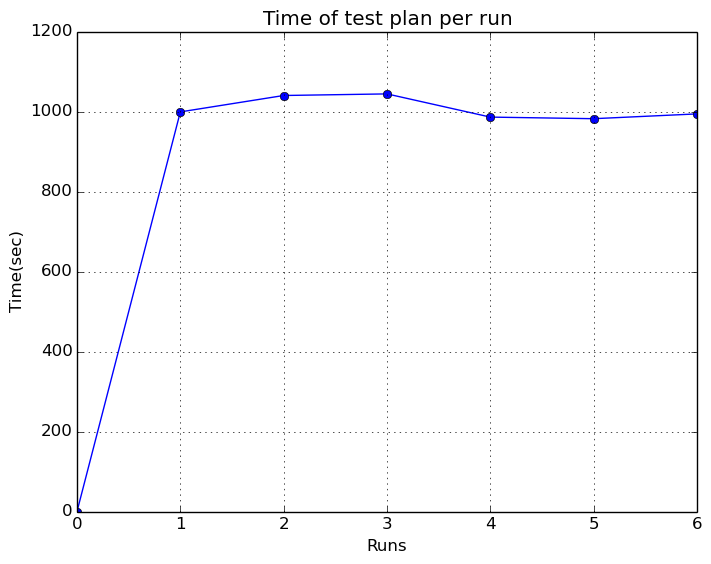
\includegraphics[width=0.75\linewidth]{../figures/nextcloud/time.png}
   \caption{Nextcloud: Time of test plan per run}
\end{figure}
\hfill\break

All of the projects in their time graphs reach a peak at the first or second run and then they all follow a downward trend, each one at its own rate. However, the fall in all cases is smooth.

The reason why the first runs of the test plan take more time, is not relevant to SecureWilly, but it derives from the time it takes to pull the images from DockerHub in the first run, as well as memory caching on data. Similarly, the rate of the fall that comes after the highest point depends on the usage of data and volumes in services and if they remain in cache memory.

It follows that the test plan is not affected by the AppArmor profiles, either they are set to complain or enforce mode. This behaviour was expected, since in the computational complexity, the AppArmor profile addition was represented by a constant.

\section{Functionality}
\underline{Enforce mode}
\hfill\break

Testing SecureWilly's functionality is actually equal to testing the input docker project, with the profiles produced set to enforce mode and evaluate if the actions described in the test plan are allowed.

The profiles produced by SecureWilly rely completely on the test plan that the user gives as input, as there is no other way to predict what actions should be allowed.  

SecureWilly performs a functionality testing inside the dynamic parser's loop, by enforcing the profiles after there are no more logs in the complain mode, and runs the test plan one more time. If there are still system logs denying actions of the test plan and new rules can be extracted from them, then SecureWilly repeats the complain mode procedure from the beginning. In this way, it ensures that all actions specified in the test plan are allowed.

Figures 5.10, 5.11 and 5.12 show each project's line graphs per service, which illustrate again the amount of rules per run, but this time emphasizing whether each run sets the profiles to complain or enforce mode.

In all docker projects, only one run of enforce mode was performed and the fact that no system logs denying actions were produced means that the test plan was executed successfully, with all of its operations allowed.

\hfill\break

\begin{figure}[h!]
  \centering
   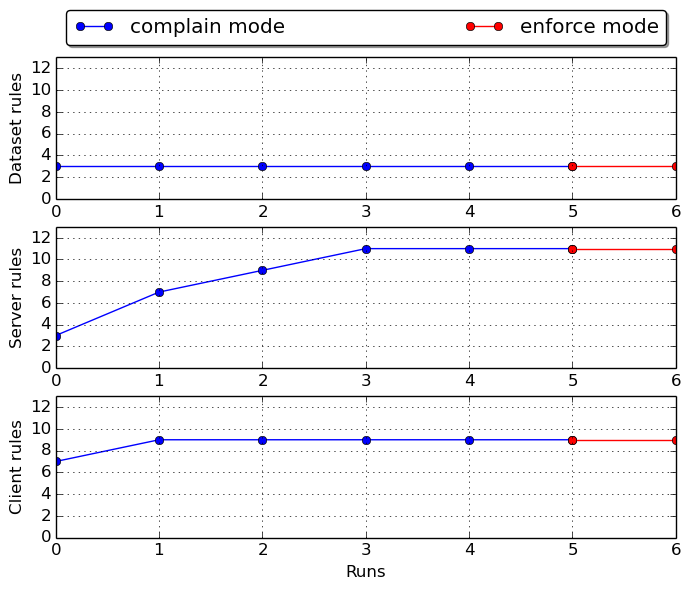
\includegraphics[width=0.8\linewidth]{../figures/mediastreaming/complain_enforce_rules.png}
   \caption{Media Streaming: Rules per run, emphasizing complain/enforce mode}
\end{figure}

\hfill\break

\begin{figure}[h!]
  \centering
   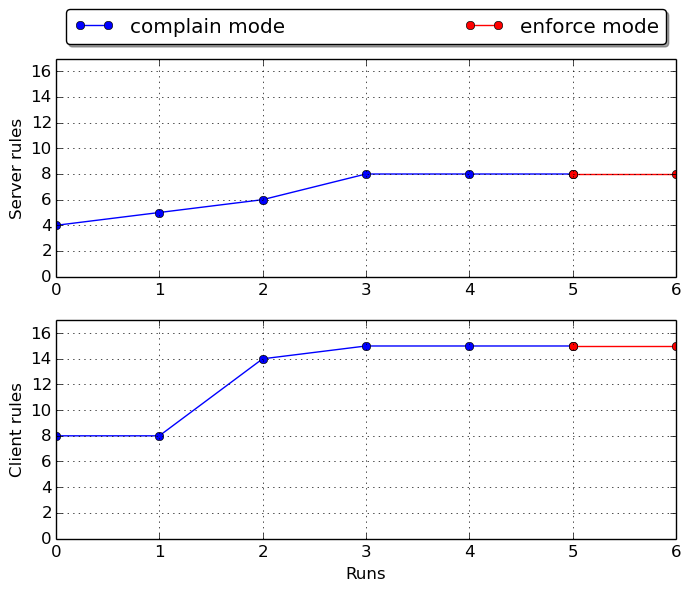
\includegraphics[width=0.75\linewidth]{../figures/datacaching/complain_enforce_rules.png}
   \caption{Data Caching: Rules per run, emphasizing complain/enforce mode}
\end{figure}

\begin{figure}[h!]
  \centering
   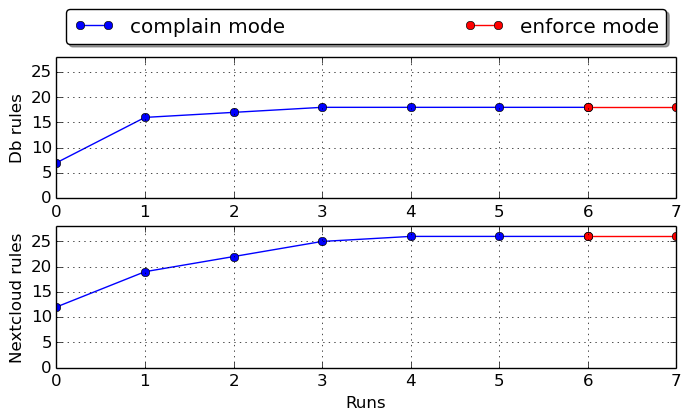
\includegraphics[width=0.75\linewidth]{../figures/nextcloud/complain_enforce_rules.png}
   \caption{Nextcloud: Rules per run, emphasizing complain/enforce mode}
\end{figure}
\hfill\break
\hfill\break
\underline{Types of rules}
\hfill\break

Another way to test the functionality of SecureWilly is to monitor the rules of each profile, identify which types of rules are encountered in it and make sure they correspond to the role and operations of each service.

\begin{textblock*}{18cm}(0.1cm,7cm) % {block width} (coords)
\begin{figure}
  \begin{minipage}[H!]{0.5\textwidth}
    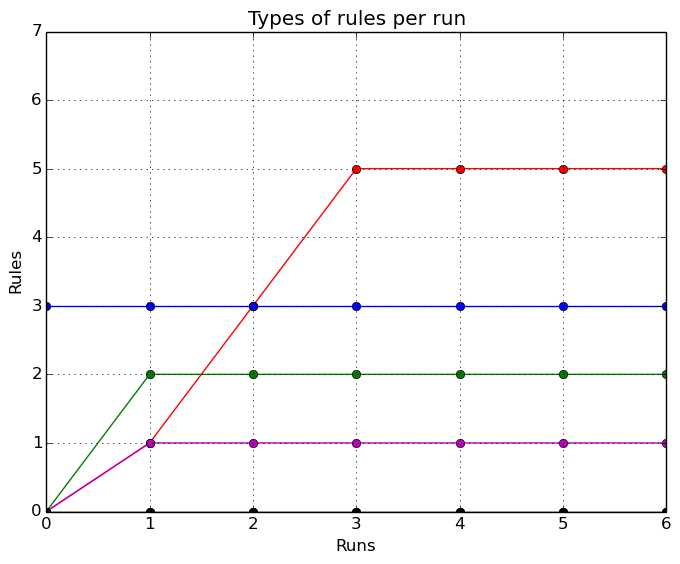
\includegraphics[width=\textwidth]{../figures/mediastreaming/nolegend/types_cloudsuitemedia-streamingserver.png}
    \caption{Media Streaming: Server types}
  \end{minipage}
  \begin{minipage}[H!]{0.5\textwidth}
    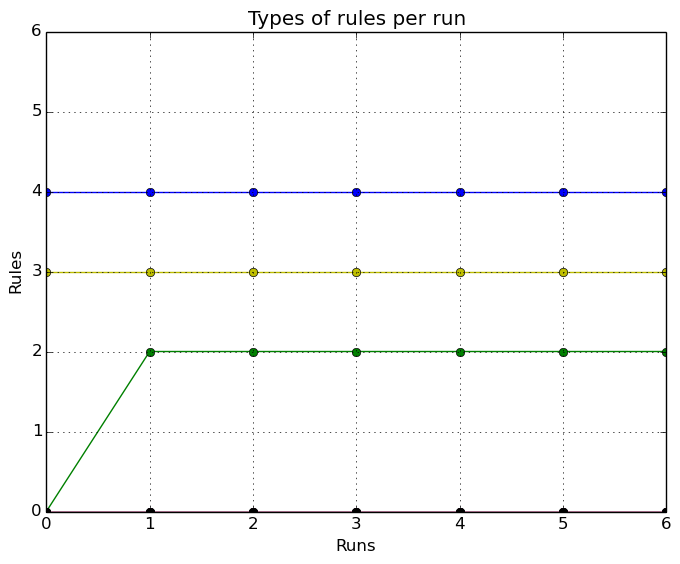
\includegraphics[width=\textwidth]{../figures/mediastreaming/nolegend/types_cloudsuitemedia-streamingclient.png}
    \caption{Media Streaming: Client types}
  \end{minipage}
\end{figure}
\end{textblock*}

\hfill\break\hfill\break\hfill\break\hfill\break\hfill\break\hfill\break\hfill\break\hfill\break\hfill\break\hfill\break\hfill\break\hfill\break\hfill\break\hfill\break\hfill\break\hfill\break\hfill\break\hfill\break

\begin{figure}[h!]
  \centering
   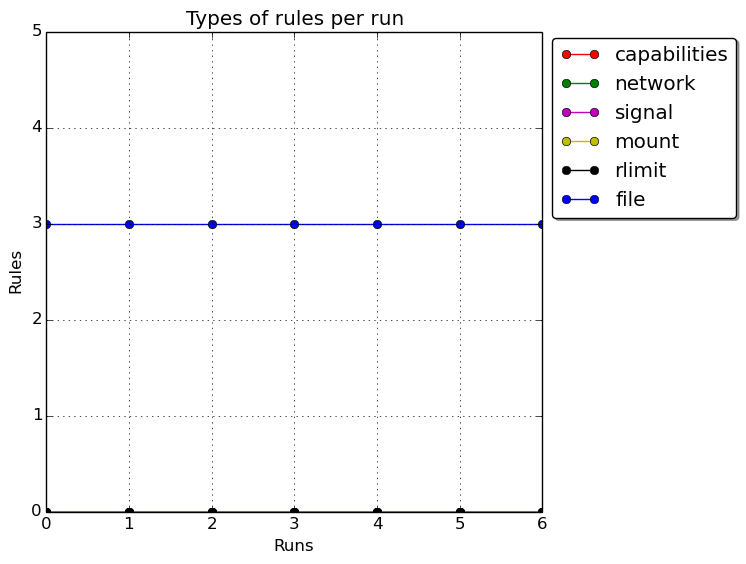
\includegraphics[width=0.7\linewidth]{../figures/mediastreaming/types_cloudsuitemedia-streamingdataset.png}
   \caption{Media Streaming: Dataset types}
\end{figure}

Figures 5.13, 5.14 and 5.15 show the line graphs of the types of different rules used in the media streaming services' profiles over runs. 

The above graphs show that each profile describes perfectly the role of the service and the operations of its task.

In server's profile, the graph shows that a server has more capability rules than other types. This derives from the fact that a server commits several actions in order to serve the clients, and thus it is expected to need some capabilities. It is evident now that capabilities are the type of rules that most of the times set the threshold, as they appear to escalate gradually on each run. The file rules can derive from file accesses the server needs, but not from volumes since there are no mount rules extracted. Network rules are extracted for the internal communication of the services and lastly, there is one signal rule, which is needed in order to send a SEGKILL/SIGTERM to the server, since it is running as a daemon.

In client's profile, it appears that client handles some volumes, since there are mount rules and the corresponding file rules. File rules are more, because the preliminary profile's rules are added to them. Moreover, client also needs some network rules in order to communicate with the server.

As it is expeted, dataset only needs some file rules which are the ones of the preliminary profile, as its container will not commit any actions.

In figures 5.16 and 5.17 we observe how server and client act in data caching example. 

It appears that plenty of network and file rules are included in server's profile, since network is needed in order to communicate with client and file rules derive from the fact that server in data caching benchmark handles a twitter dataset. Apart from these types, it needs only one signal rule in order to be able to terminate.

As for the client, network rules are needed in order to make requests to the server while the rest of the rules are all relevant to the way we implemented this example. Mount and file rules derive both from the volume script we used in order to run this benchmark non-interactively, while all the signal rules derive from the timeout and kill signals - either sent by the client or received by one of its process - which were used to stop all processes of clients when the benchmarking was complete.

Lastly, figures 5.18 and 5.19 represent Nextloud's line graphs, one for the database service and one for the server - nextcloud.

In these graphs, it is more clear than ever that Nextcloud is the most complex of the examples used, as its profiles consist of a variety of rules. 

Starting with nextcloud service, capability rules, which is the type with the most rules in the profile, escalate gradually per run and they are responsible for setting the threshold at run four, exactly like we observed in media streaming. This is reasonable, since Nextcloud's server requires several capabilities in order to connect to the database and serve all of its users.  File and mount rules are added by static analysis, deriving from the volumes mounted which we described in nextcloud's section, and remain stable for the rest of the runs. Some network rules are needed, like in almost every multi-service project, in order to communicate with the database, as well as some signal rules in order to make the server capable of getting terminated, rather than becoming a zombie container process.

Database's service needs some capability rules as well, fewer than the server though. It needs some signal rules in order to be able to handle termination signals, sent and received, as well as some network rules that constitute the communication with the server possible. However, the profile mainly consists of mount and file rules, due to the volumes it handles and the file accesses it needs to make, which is a fundamental characteristic of a database.
 
\begin{figure}[h!]
  \centering
   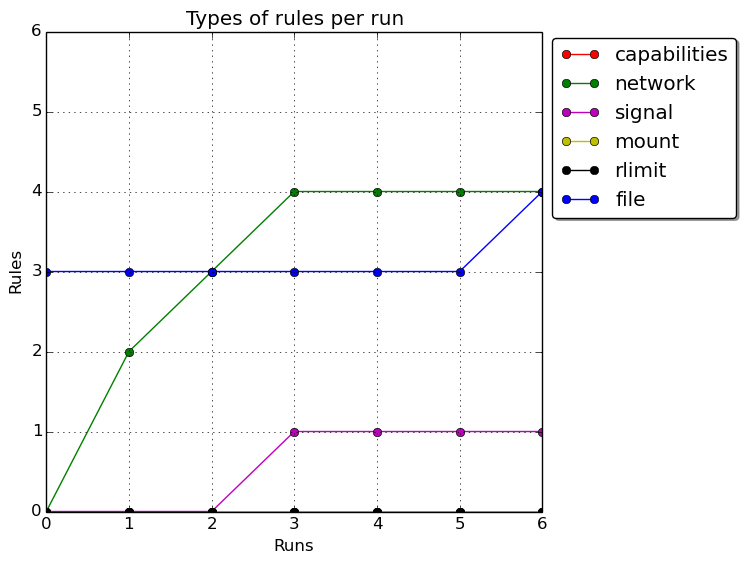
\includegraphics[width=0.65\linewidth]{../figures/datacaching/types_cloudsuitedata-cachingserver.png}
   \caption{Data Caching: Server types}
\end{figure}

\begin{figure}[h!]
  \centering
   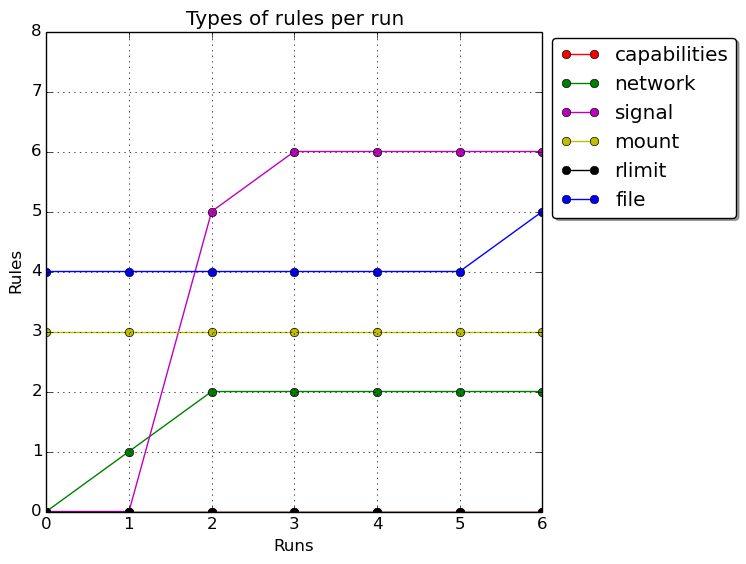
\includegraphics[width=0.65\linewidth]{../figures/datacaching/types_cloudsuitedata-cachingclient.png}
   \caption{Data Caching: Client types}
\end{figure}

\begin{figure}[h!]
  \centering
   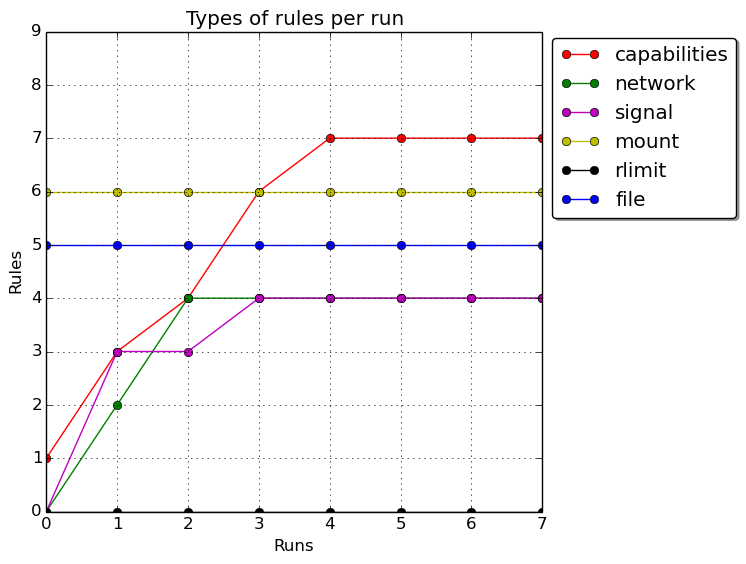
\includegraphics[width=0.68\linewidth]{../figures/nextcloud/types_nextcloud.png}
   \caption{Nextcloud: Nextcloud types}
\end{figure}

\begin{figure}[h!]
  \centering
   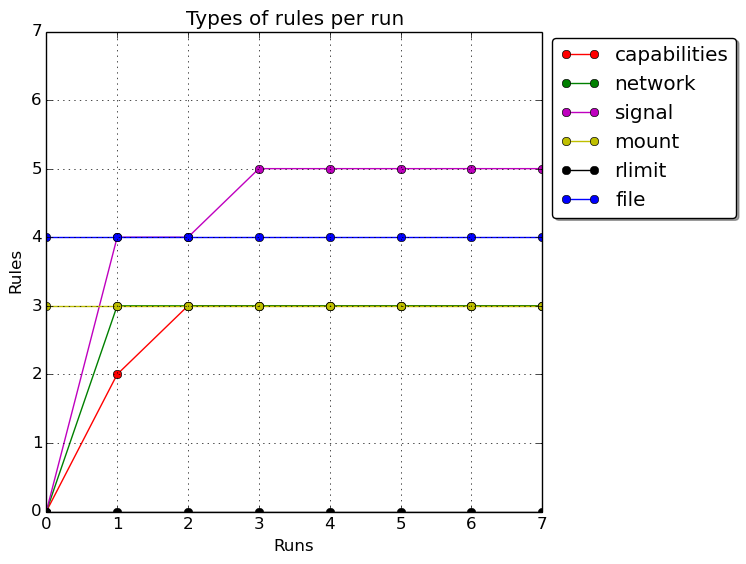
\includegraphics[width=0.68\linewidth]{../figures/nextcloud/types_db.png}
   \caption{Nextcloud: Db types}
\end{figure}
In the light of the above, it is clear that the AppArmor profiles that are produced by SecureWilly are adjusted completely to the docker project and are closely tied with their tasks. This means they are efficient and secure, since they allow any docker project to run unhinderedly, but all redundant actions will be blocked.\\

\section{Scalability}
\subsection{Multiple services}
SecureWilly should be able to handle large increases in services and other workloads. 

In order to evaluate scalability we perfomed a testing using media streaming benchmark with multiple clients.

Figure 5.20 illustrates a line graph which shows the execution time of test plan per run for each test case. As it is expected, time has a steady increase, accordingly with the augmentation of the amount of clients.

\begin{figure}[h!]
  \centering
   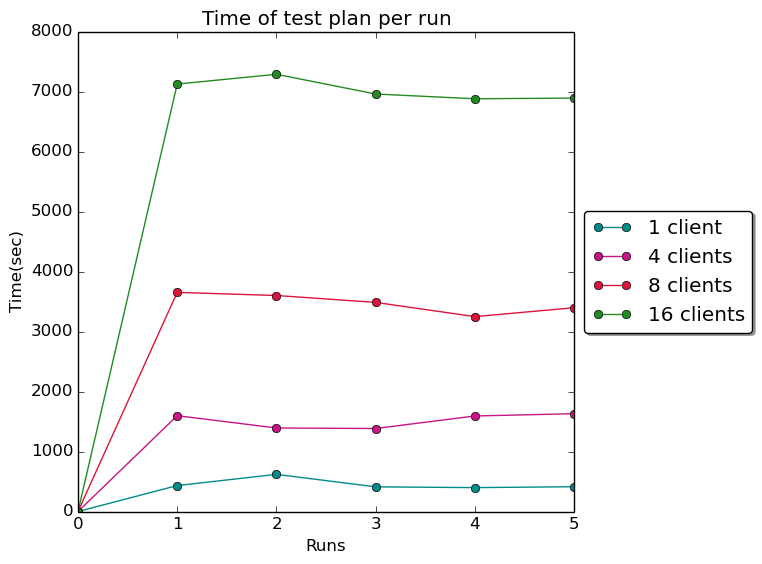
\includegraphics[width=0.8\linewidth]{../figures/scalability/time1_4_8_16.png}
   \caption{Media Streaming: Time of test plan per run for each test case}
\end{figure}

However, as we previously described, the correct way to measure the performance per case is not time but runs.

In figures 5.21 and 5.22, the line graphs representing rules per run for the test cases of 4 and 8 clients (the figure about the 16 clients test case was left out, because the line graphs were identical) respectively, show that the amount of total runs executed is not affected at all by the increase in the amount of clients and neither does the threshold. Moreover, since clients are running the same docker run command, their lines follow exactly the same trend.

\begin{figure}[h!]
  \centering
   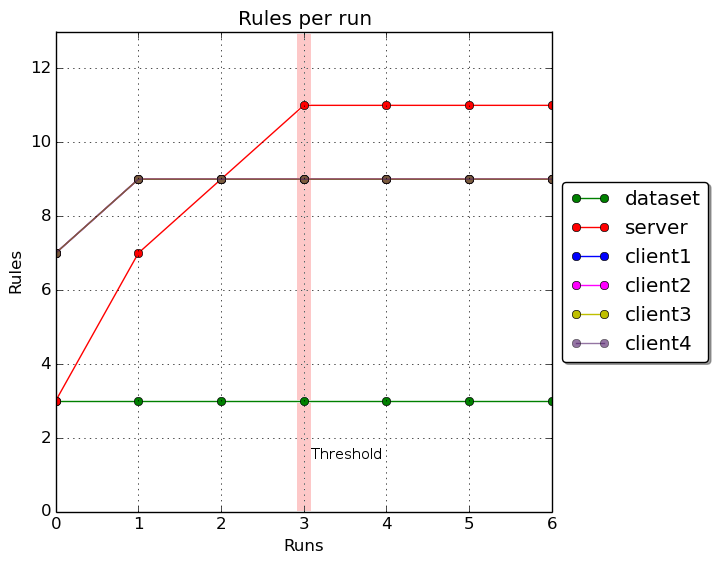
\includegraphics[width=0.65\linewidth]{../figures/scalability/rules_4_t.png}
   \caption{Media streaming with 4 clients}
\end{figure}
\hfill\break\hfill\break
\begin{figure}[h!]
  \centering
   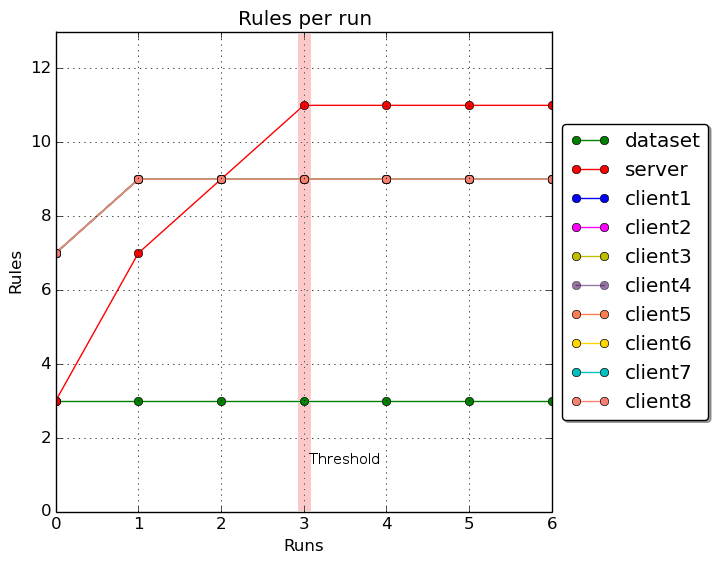
\includegraphics[width=0.68\linewidth]{../figures/scalability/rules_8_t.png}
   \caption{Media streaming with 8 clients}
\end{figure}

Therefore, it has been proved that SecureWilly can handle large scale projects and its task is not affected in any way by them.

\subsection{Distributed systems}
The multiple services we have examined up to this point were all running on the same machine. The scalability of SecureWilly would make more sense if the multiple services were distributed on different machines.

This option addresses distributed systems and is not yet implemented on SecureWilly. However, the way SecureWilly approaches the services and their profiles constitutes this option implementable.

Services are already considered as distignuished components of a docker project by SecureWilly and each one of them is restricted at a different rate by a private profile. The only thing that is shared is the kernel and the system logs it produces. In case of different machines, the system logs will exist on different systems. Therefore, one approach to handle this would be to implement requests to each machine/node from the machine where SecureWilly is running about sending the respective system logs to this machine. After SecureWilly's processing, the respective profile would be sent to the machine/node on which each service will run.

\begin{figure}[h!]
  \centering
   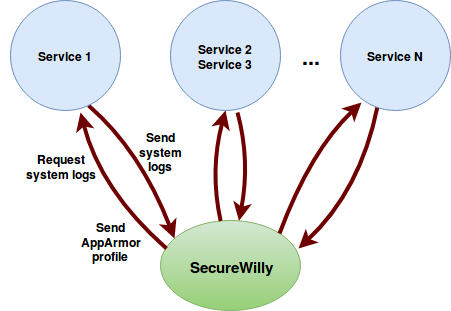
\includegraphics[width=0.68\linewidth]{../figures/DistributedSystems.png}
   \caption{SecureWilly handling distributed services}
\end{figure}

\section{Summary}
To sum up, the profiles produced by SecureWilly are service-oriented but it is recommended to run SecureWilly on a system because each machine could cause slight differences to the profiles.

AppArmor's overhead has proved to be very small and therefore, AppArmor is still very beneficial for an application to harden its security.

All in all, SecureWilly has proved through experimental evaluation that is functional and produces profiles which reach their fundamental goal, and scalable as well, meaning it can handle large increases in services. Furthemore, the performance is exactly as it is expected by its computational complexity and it depends on the performance of the test plan, as SecureWilly does not add any great delays.

In order to perform these testings, SecureWilly used some demanding benchmarks of CloudSuite and also Nextcloud, which is a widely used real software, and the profiles produced by SecureWilly could constitute a useful contribution to the community of Nextcloud.
